\documentclass[a4paper,11pt]{article}
%
\usepackage[UKenglish]{babel}
\usepackage{graphicx}
\usepackage{amsmath}
\usepackage{float}
\usepackage{listings}
\usepackage{dtsyntax}
\usepackage{svg}
\usepackage{verbatim}
%
\restylefloat{figure}
\DeclareGraphicsExtensions{.png,.jpg}
%
%
%opening
\title{OpenHPL - Correction of pipe model}
\author{BB}
%
\begin{document}
\lstset{language=modelica} 	

\maketitle



\begin{abstract}
The OpenHPL class \texttt{Pipe} implements a rigid water pipe model. The current implementation have certain issues. In the following note a revision is proposed.
This includes a class of test cases.
\end{abstract}
%
\tableofcontents
%
\section{Introduction}
%  https://docs.bentley.com/LiveContent/web/Bentley%20HAMMER%20SS6-v1/en/GUID-F87F1515-85CE-4FF3-9C5F-3AD5E427F125.html
%  https://ocw.snu.ac.kr/sites/default/files/NOTE/HD%20Ch6-LC9.pdf
% 
In the following transient change of pressure in a pipe is discussed. When the change is slow compared to the speed of sound, the elastic pressures waves in the medium can be ignored. This approach is often denoted rigid water column and implies that the instantaneous flow rate is constant in all cross sections in the pipe
\footnote{Since the compressibility of the medium is assumed to be constant, the density and hence the mass flow is also constant in all cross sections.}.
The rigid water column momentum equation can be derived from Newtons first law:
\[
F=m\cdot a
\]
Writing out this relation for the pipe in figure \ref{fig:pipe} yields
\[
\left(p_{1}+\rho \cdot g \cdot H \right)\cdot A_{1} - p_{2}\cdot A_{2} -F_{f} = \left(\rho\cdot \overline{A} \cdot L \right) \frac{dv}{dt}
\]
where $F_{f}$ is the total friction force along the pipe and $\overline{A} $ is the average area such that the total mass of water $M$ is $M=\overline{A} \cdot L$ (see also \ref{sec:d_and_a})).
% loss for a straight pipe with reference diameter $\tilde{D}$ and $F_{c}$ is the additional friction force due to the change in diameter.
Since OpenHPL is formulated with the mass flow $m=\rho \cdot q =\rho \cdot A \cdot v$ the above can be rewritten as
\[
\left(p_{1}+\rho \cdot g \cdot H \right)\cdot A_{1} - p_{2}\cdot A_{2} - F_{f}= L \cdot \frac{dm}{dt}
\]
\subsection{Friction force}
%
In principle the friction force is found by integrating the wall shear force $\tau_{w}$ along the all surfaces. For constant diameter pipe the traditional approach is to express this friction loss through the semi-empirical head loss formula 
\[
F_{f}= A \cdot \rho \cdot  g \cdot h_{f}= A \cdot \rho \cdot g \left[ f  \cdot \left(\frac{L}{D}\right) \frac{v^{2}}{2g} \right]
\]
where $f$ is the friction factor, commonly taken from the Moody diagram or various approximations to the Moody diagram 
%
\begin{figure}[H] % The figure environment allows for captioning and floating
	\centering % Centers the image within the figure environment
	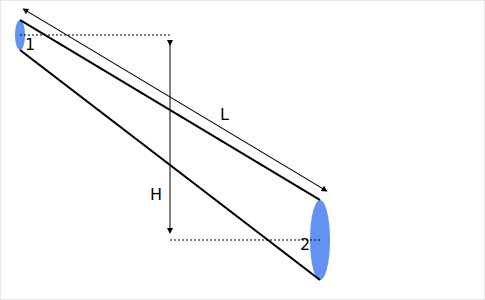
\includegraphics[width=0.9\textwidth]{01_pipe.png} 
	\caption{Consider a pipe with inlet diameter $D_1$ and outlet diameter $D_2$ and length $L$.} % Caption for the image
	\label{fig:pipe} % Label for cross-referencing
\end{figure}
%
\subsection{Area change/conical pipe}
%
If the pipe is strongly conical (either diverging or converging) special loss models must be used as the

\section{Today's implementation}
\begin{comment}
\begin{lstlisting}
within OpenHPL.Waterway;
model Pipe "Model of a pipe"
outer Data data "Using standard data set";
extends OpenHPL.Icons.Pipe;
extends OpenHPL.Interfaces.ContactPort;

// Geometrical parameters of the pipe:
parameter SI.Length H = 25 "Height difference from the inlet to the outlet" annotation (
Dialog(group = "Geometry"));
parameter SI.Length L = 6600 "Length of the pipe" annotation (
Dialog(group = "Geometry"));
parameter SI.Diameter D_i = 5.8 "Diameter of the inlet side" annotation (
Dialog(group = "Geometry"));
parameter SI.Diameter D_o = D_i "Diameter of the outlet side" annotation (
Dialog(group = "Geometry"));
parameter SI.Height p_eps (displayUnit = "mm") = 1e-5 "Pipe roughness height" annotation (
Dialog(group = "Geometry"));
parameter Real K_c = 0.1 "Loss coefficient for contraction"
annotation (Dialog(group = "Geometry"));
// Steady state:
parameter Boolean SteadyState=data.SteadyState "If true, starts in steady state" annotation (Dialog(group="Initialization"));
parameter SI.VolumeFlowRate Vdot_0=data.Vdot_0 "Initial flow rate of the pipe" annotation (Dialog(group="Initialization"));

SI.Diameter D_ = 0.5 * (D_i + D_o) "Average diameter";
SI.Mass m "Water mass";
SI.Area A_i = D_i ^ 2 * C.pi / 4 "Inlet cross-sectional area";
SI.Area A_o = D_o ^ 2 * C.pi / 4 "Outlet cross-sectional area";
SI.Area A_ = D_ ^ 2 * C.pi / 4 "Average cross-sectional area";
Real cos_theta = H / L "Slope ratio";
SI.Velocity v "Water velocity";
SI.Velocity v_o "Outlet water velocity";
SI.Force F_f "Friction force";
SI.Force F_taper "Taper friction force"; 
SI.Momentum M "Water momentum";
SI.Pressure p_i "Inlet pressure";
SI.Pressure p_o "Outlet pressure";
SI.Pressure dp=p_o-p_i "Pressure difference across the pipe";
SI.VolumeFlowRate Vdot(start = Vdot_0) "Volume flow rate";



protected
parameter SI.Diameter D_eff=
if D_i == D_o then
D_i
else
(D_i - D_o) / log(D_i/D_o) "Effective diameter for a linear taper";

initial equation
if SteadyState then
der(M) = 0;
end if;
equation
Vdot = mdot / data.rho "Volumetric flow rate through the pipe";
v = Vdot / A_ "Average water velocity";
v_o = Vdot / A_o "Outlet water velocity";
M = data.rho * L * Vdot "Momentum of water";
m = data.rho * A_ * L "Mass of water";
F_f = Functions.DarcyFriction.Friction(v, D_eff, L, data.rho, data.mu, p_eps)
"Friction force";
F_taper = K_c * 0.5 * data.rho * A_o * v_o * abs(v_o)
"Tapering (local contraction) loss";
der(M) = data.rho * Vdot^2 * (1/A_i - 1/A_o)
+ p_i * A_i - p_o * A_o
- F_f - F_taper
+ m * data.g * cos_theta
"Momentum balance including tapering loss";
p_i = i.p "Inlet pressure";
p_o = o.p "Outlet pressure";


end Pipe;


\end{lstlisting}
\end{comment}

%

\section{New implementation}

Overall goal and checks:
\begin{enumerate}
	\item When inlet and outlet diameter is the same, should be identical to "simple pipe"
	\item 
\end{enumerate} 
%
\section{Future development}
%
\bibliographystyle{plain}
\bibliography{ohpl}
%
\appendix
%
\section{On diameter and area}
\label{sec:d_and_a}
%
Consider the pipe in figure \ref{fig:pipe_apendix} with inlet and outlet diameter $D_1$ and $D_2$. The corresponding areas are $A_1$ and $A_2$.
The average diameter $\overline{D}$ is 
\[
\overline{D}=\frac{1}{2}\left(D_1 + D_2\right)
\]
The average area $\overline{A}$ is
\[
\overline{A}=\frac{1}{2}\left(A_1 + A_2\right)
\]
Since the area is a quadratic function of diameter, the mean area $\overline{A}$ is different than the area of the mean diameter. In the model 
\[
\tilde{D}=\sqrt{\frac{4}{\pi}\overline{A}}
\]
%
\subsection{Further details}
%
%
Introducing $D_1=D$ and $D_2=\delta \cdot D$, the average diameter can be written as
%
\[
\overline{D}=\frac{\left(1+\delta\right)}{2}\cdot D
\]
%
The average area can be written as
%
\[
\overline{A}=\frac{\pi}{4}\cdot D^{2} \cdot \frac{\left(1 +\delta^{2}\right)}{2}
\]
%
The area, based on the average diameter can be written as
\[
A\left(\overline{D}\right)=\frac{\pi}{4}\cdot D^{2}\cdot \frac{\left(1+2\delta+\delta^2\right)}{4}
\]
\[
A\left(\overline{D}\right)=\frac{\pi}{4}\left(\frac{1}{2}\left(D_1 + D_2\right)\right)^{2}=\frac{\pi}{4}\cdot\frac{1}{4}\left(D_{1}^{2} + 2 D_{1} D_{2} + D_{2}^{2}\right)=
\]




%
\begin{figure}[H] % The figure environment allows for captioning and floating
	\centering % Centers the image within the figure environment
	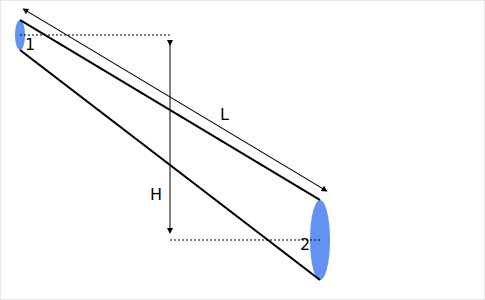
\includegraphics[width=0.9\textwidth]{01_pipe.png} 
	\caption{Consider a pipe with inlet diameter $D_1$ and outlet diameter $D_2$ and length $L$.} % Caption for the image
	\label{fig:pipe_apendix} % Label for cross-referencing
\end{figure}
%
\subsection{Friction loss of variable area pipe}
%
In general it is difficult to find a closed form equation for the friction force for a pipe with varying area that is completely universal.
%
\[
F_{f}= A \cdot \rho \cdot  g \cdot h_{f}= A \cdot \rho \cdot g \left[ f \cdot \left(\frac{L}{D}\right) \frac{v^{2}}{2g} \right] =\frac{1}{A} \cdot \rho \cdot g \left[ f \left(\frac{L}{D}\right) \frac{Q^{2}}{2g} \right]
\]
 Assuming a linear diameter distribution from the inlet to the outlet
 \[
 D\left(x\right)=D_{1}+\frac{\left(D_{2}-D_{1} \right)}{L}\cdot x
 \]
 or
 \[
  D\left(x\right)=D_{1}+\frac{\left(D_{2}-D_{1} \right)}{L}\cdot x
 \]
%
 In principle the friction factor $f$ is a function of the Reynolds number $Re$ and relative roughness $\epsilon/D$. Ignoring this, and setting both to the constant value based on the mean value
 
%
%
\bibliographystyle{plain}
\bibliography{ohpl}
\end{document}